\RequirePackage{plautopatch}
\documentclass[dvipdfmx,a4paper]{jsarticle}
\usepackage{graphicx}

\usepackage{amsmath}
\usepackage{amssymb}
\usepackage{float}

\title{Day2 課題}
\author{古賀 光一朗}
\date{2025年6月23日 ~ 2025年6月30日}

\begin{document}
    \maketitle
    \begin{figure}[H]
        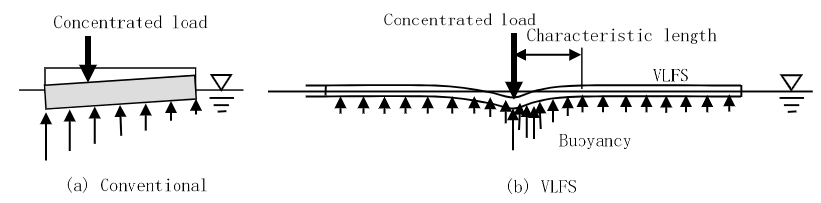
\includegraphics[width=1\linewidth]{summer/fluid-tructure-interactions/day2.01.png}
        \caption{Caption}
        \label{fig:enter-label}
    \end{figure}
    前回の授業で“弾性支床上の梁モデル“について検討した。ここで,$EI$ は単位幅あたりの曲げ剛性を,$k_r$ は単位面積当たりの復原力係数を表す。浮体中央に原点を取る。
    \begin{equation}
        EI\frac{d^4W}{dx^4}+k_rW=f
    \end{equation}
    (1) 式(*)の斉次解が以下で与えられることを確認しなさい(復習,合計4つ)。αの定義については前回の資料を参照。
    \begin{equation}
        W_1 = \exp{\frac{ax}{\sqrt{2}}}\cos{\frac{ax}{\sqrt{2}}}, 
        W_2 = \exp{\frac{ax}{\sqrt{2}}}\sin{\frac{ax}{\sqrt{2}}}, 
        W_3 = \exp{\frac{-ax}{\sqrt{2}}}\cos{\frac{ax}{\sqrt{2}}}, 
        W_4 = \exp{\frac{-ax}{\sqrt{2}}}\sin{\frac{ax}{\sqrt{2}}}
    \end{equation}
    中央部に荷重$P$が作用した場合(荷重$f=P\cdotp \delta(x=0)$ , デルタ関数$\delta$は積分すると$1$になる), 一般解は上記の斉次解の線形結合,つまり
    $$W=a_1W_1+a_2W_2+a_3W_3+a_4W_4$$
    で得られる。

    
$$\space$$
    (2) 事象が左右に対称と考えて,右半分の領域について考えよう。未知の係数$a_1,a_2,a_3,a_4$は適当な条件を付することで与えられる。今回の場合,付するべき条件は次のようになる。下の4つの式の物理的な意味をそれぞれ与えなさい。
    \begin{equation}
        \frac{d^2w}{dx^2}=0,\ \text{at}\ x=\infty
    \end{equation}
    \begin{equation}
        \frac{d^3w}{dx^3}=0,\ \text{at}\ x=\infty
    \end{equation}
    \begin{equation}
        \frac{dw}{dx}\ \text{at}\ x=0
    \end{equation}
    \begin{equation}
        \int_0^{L/2}k_rwdx=\frac{P}{2}
    \end{equation}
    例) “浮体の右端が自由端であることからモーメントがゼロになる。モーメントは曲率に曲げ剛性を乗じたものであり,式(3)は曲率ゼロ=右端でモーメントがゼロ“

$$\space$$
    
    (3) (1)の斉次解のうち,$x=\infty$での境界条件を満たすものは,$W_3,W_4$である。特徴を調べるために$W_3$の形状を描きなさい。エクセルなどのツールを使って構わない。ここでは$\frac{a}{\sqrt{2}}=1$としてよい。
    
$$\space$$
    ここからは具体的にポンツーン型メガフロートの場合を考えてみる。メガフロートの構造は巨視的には図の〇を付けた二重底部分と類似である。



    (4) 実際の$a$の値がどの程度になるか考えてみる。板厚$t$の二つの板(上側とした側,デッキとボトム)の間の間隔が$H$と考えるとメガフロートの単位幅当たりの断面二次モーメントは,近似的に
    \begin{equation}
        I=\frac{H^2}{2}t
    \end{equation}
    で与えられる。これを説明しなさい。実際には縦隔壁などが存在するので,式(7)は断面二次モーメントの下限の推定値を与える。

    \begin{figure}[H]
        \centering
        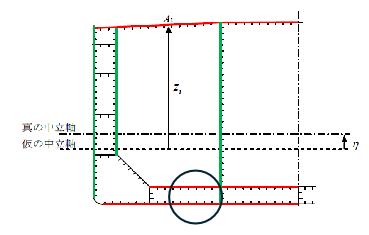
\includegraphics[width=0.8\linewidth]{summer/fluid-tructure-interactions/day2.02.png}
        \caption{Caption}
        \label{fig:enter-label}
    \end{figure}


    (5) 板厚が$t=20mm(=0.02m)$程度,$H=4m$と考えたときの曲げ剛性 ($=EI,E=\text{スチールの弾性係数}$で $2\times10^{11}\ N/m^2$の値を計算し,さらにポンツーン型浮体の(単位面積当たり)復原力係数は$k_r=9800\  N/m^3$であることから,$\frac{\sqrt{2}}{\alpha}$の値を求めなさい。
    

    (6) (3)で描いた図を$x$軸方向に$\frac{\sqrt{2}}{\alpha}$倍すると,メガフロートの変形になる。この点で$\alpha$は縮尺係数のようなものである。このことを念頭において,特性距離$\lambda_s=2\pi\sqrt[4]{\frac{EI}{k_r}}$はどのような物理的意味があるかを述べなさい。

    
\end{document}
